\chapter{\label{chap:anforderungen}Anforderungsdefinition}
Dieses Kapitel beschreibt die Anforderungen an eine Offline First Anwendung unter Berücksichtigung von Funktionalität, Konfliktmanagement und der Bedienoberfläche.
Aus den oben genannten \hyperref[chap:szenarien]{Szenarien} werden im Folgenden die Anforderungen hergeleitet, die eine offlinefähige Anwendung erfüllen soll.
%
% User-Stories
%
\section{User-Stories}
Aus den in Kapitel \ref{chap:szenarien} erarbeiteten Szenarien ergeben sich die folgenden User-Stories, die von der offlinefähigen Adressbuchanwendung erfüllt werden sollen.
Ein Ziel der Arbeit ist es, EntwicklerInnen bei der Wahl einer Technologie mit der eine offlinefähige Anwendung entwickelt werden kann, zu unterstützen.
Deswegen werden zunächst die Anforderungen aus Sicht der NutzerInnen definiert, danach die aus Entwicklingsperspektive.
\sub{User Perspektive}
Die folgende \hyperref[tab:user]{Tabelle} zeigt die Software-Anforderungen an eine offlinefähige Kontaktliste aus der NutzerInnenperspektive.
\begin{longtable}[c]{@{}
>{\columncolor[HTML]{CFFCC2}}l ll@{}}
\toprule
    \multicolumn{1}{p{0.15\textwidth}}{\cellcolor[HTML]{cffcc2}\textbf{ID}}
    & \multicolumn{1}{p{0.85\textwidth}}{\cellcolor[HTML]{cffcc2}\textbf{Anforderung aus Userperspektive}}\\ \hline
\endfirsthead
%
\endhead
%
  \multicolumn{1}{l}{\cellcolor[HTML]{cffcc2}\textbf{User-Story 1}} &
  \multicolumn{1}{p{0.85\textwidth}}
  {Ich als NutzerIn möchte die Anwendung immer und überall, auch ohne Internetzugang zu nutzen.}\\
  \midrule
  %
  \multicolumn{1}{l}{\cellcolor[HTML]{cffcc2}\textbf{User-Story 2}} &
  \multicolumn{1}{p{0.85\textwidth}}
  {Ich als Nutzerin möchte, dass die Kontaktliste schnell und effizient geladen wird, um Zeit zu sparen.}\\
  \midrule
  %
  \multicolumn{1}{l}{\cellcolor[HTML]{cffcc2}\textbf{User-Story 3}} &
  \multicolumn{1}{p{0.85\textwidth}}
  {Ich als NutzerIn möchte jeden Kontakteintrag finden, um zu wissen ob ich ihn schon gespeichert habe.}\\
  \midrule
  %
  \multicolumn{1}{l}{\cellcolor[HTML]{cffcc2}\textbf{User-Story 4}} &
  \multicolumn{1}{p{0.85\textwidth}}
  {Ich als NutzerIn möchte Einträge immer und überall, auch ohne Internetzugang, erstellen, editieren oder löschen können, um meine Liste zu verwalten.}\\
  \midrule
  %
  \multicolumn{1}{l}{\cellcolor[HTML]{cffcc2}\textbf{User-Story 5}} &
  \multicolumn{1}{p{0.85\textwidth}}
  {Ich als NutzerIn möchte keine in der Anwendung gespeicherten Daten verlieren.}\\
  % end
  \bottomrule \cellcolor[HTML]{FFFFFF}
  \vspace{0.1cm}\\
  \noalign{\hspace{0.0525\textwidth}\grayRule}
  \caption{Anforderungen aus Userperspektive}
  \label{tab:user}\\
\end{longtable}

% Das in Abbildung \ref{fig:uc} gezeigte Use-Case-Diagramm veranschaulicht die in der obigen Tabelle \ref{tab:uc} aufgeführten Anwendungsfälle.
% \begin{figure}[H]
%     \centering
%     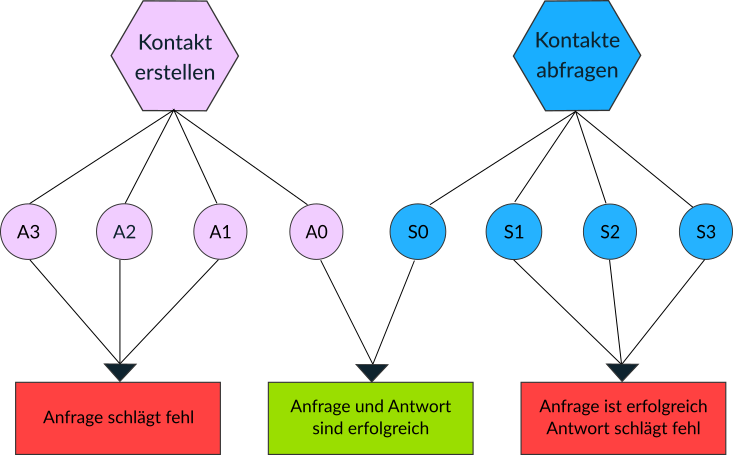
\includegraphics[width=0.4\textwidth]{Szenarien}
%     \grayRule
%     \caption[Use-Case Diagramm]{Platzhalter für US-Diagramm}
%     \label{fig:uc}
% \end{figure}
\sub{Developer Perspektive}
Die folgende Tabelle zeigt die Software-Anforderungen an eine offlinefähige Kontaktliste aus der EntwicklerInnenperspektive.
\begin{longtable}[c]{@{}
>{\columncolor[HTML]{CFFCC2}}l ll@{}}
\toprule
  \multicolumn{1}{p{0.15\textwidth}}{\cellcolor[HTML]{cffcc2}\textbf{ID}}
  & \multicolumn{1}{p{0.85\textwidth}}{\cellcolor[HTML]{cffcc2}\textbf{Anforderung aus Entwicklungsperspektive}}\\ \hline \noalign{\vskip 0.1cm}
\endfirsthead
%
\endhead
%
  \multicolumn{1}{l}{\cellcolor[HTML]{cffcc2}\textbf{User-Story 1}} &
  \multicolumn{1}{p{0.85\textwidth}}
  {Ich als EntwicklerIn möchte die Daten lokal und auf dem Server speichern, um deren Erreichbarkeit unabhängig vom Internetstatus zu gewährleisten.}\\
  \midrule
  %
  \multicolumn{1}{l}{\cellcolor[HTML]{cffcc2}\textbf{User-Story 2}} &
  \multicolumn{1}{p{0.85\textwidth}}
  {Ich als EntwicklerIn möchte ich nur die Adressbucheinträge oder deren Aktualisierungen laden, die sich nicht schon auf dem Endgerät befinden, um Datentraffic und Ladezeiten zu sparen.}\\
  \midrule
  %
  \multicolumn{1}{l}{\cellcolor[HTML]{cffcc2}\textbf{User-Story 3}} &
  \multicolumn{1}{p{0.85\textwidth}}
  {Ich als EntwicklerIn möchte ich jeden Eintrag identifizieren, um jedem Adressbucheintrag Operationen zuzuweisen und einzelne Kontakte zu finden.}\\
  \midrule
  %
  \multicolumn{1}{l}{\cellcolor[HTML]{cffcc2}\textbf{User-Story 4}} &
  \multicolumn{1}{p{0.85\textwidth}}
  {Ich als EntwicklerIn möchte ich jeden Eintrag versionieren, um zu wissen ob wann ein Eintrag bearbeitet wurde.}\\
  \midrule
  %
  \multicolumn{1}{l}{\cellcolor[HTML]{cffcc2}\textbf{User-Story 5}} &
  \multicolumn{1}{p{0.85\textwidth}}
  {Ich als EntwicklerIn möchte dass alle von NutzerInnen vorgenommenen Änderungen beim System ankommen und keine Daten verloren gehen.}\\
  \midrule
  %
  \multicolumn{1}{l}{\cellcolor[HTML]{cffcc2}\textbf{User-Story 6}} &
  \multicolumn{1}{p{0.85\textwidth}}
  {Ich als EntwicklerIn möchte auftretende Konflikte effizient speichern, um mit ihnen umgehen können. \todo{Mit ihnen umgehen heißt: selbstständig oder von User lösen, zum konfliktfreien Zustand gelangen}}\\
  \midrule
  %
  \multicolumn{1}{l}{\cellcolor[HTML]{cffcc2}\textbf{User-Story 7}} &
  \multicolumn{1}{p{0.85\textwidth}}
  {Ich als EntwicklerIn möchte eine Technologie verwenden die leicht zu verstehen und implemenieren ist, um den Arbeitsaufwand gering zu halten.}\\
  \midrule
  %
  \multicolumn{1}{l}{\cellcolor[HTML]{cffcc2}\textbf{User-Story 6}} &
  \multicolumn{1}{p{0.85\textwidth}}
  {Ich als EntwicklerIn möchte sauberen und verständlichen Code schreiben, um die Les-- und Wartbarkeit zu erhöhen.}\\
  % end
  \bottomrule \cellcolor[HTML]{FFFFFF}
  \vspace{0.1cm}\\
  \noalign{\hspace{0.0525\textwidth}\grayRule}
  \caption{Anforderungen aus Entwicklungsperspektive}
  \label{tab:dev}\\
\end{longtable}
%
% Das in Abbildung \ref{fig:uc} gezeigte Use-Case-Diagramm veranschaulicht die in der obigen Tabelle \ref{tab:dev} aufgeführten Anwendungsfälle.
% \begin{figure}[H]
%     \centering
%     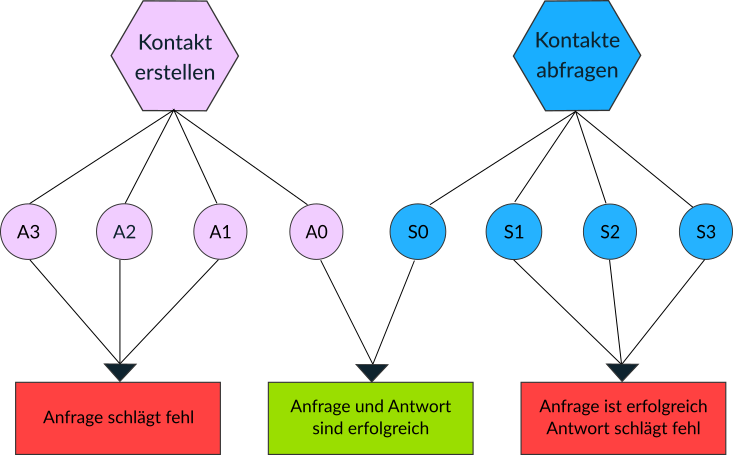
\includegraphics[width=0.4\textwidth]{Szenarien}
%     \grayRule
%     \caption[Use-Case Diagramm]{Platzhalter für US-Diagramm}
%     \label{fig:uc}
% \end{figure}
%
% Funktionalität
%
%
%
\section{Scope}
Prototypische Applikation mit den Technologien \todo{Hoodie} und Redux Offline. \todo{Begründung?}\\
Testumgebung ist mit zu entwickeln um Technologien zu testen...  Wie oft muss ich was testen? Was möchte ich für eine Aussage machen? Ich stelle folgende Fragen:
\begin{itemize}
  \item was versprechen die Technologien?
  \item Wie funktionieren die Technologien?
  \item Welche Strategie zur Konfliktlösung wird verwendet?
  \item Wie hoch ist der Implementierungsaufwand?
\end{itemize}
%
%
\section{Funktionalität}
  {Um die Anwendung auch ohne Internetzugang zu nutzen, sollen die Daten auch offline erreichbar sein.}
  {Die Daten werden auf dem Server und lokal gespeichert. Lokal bedeutet in einer lokalen Datenbank oder im Browser (localStorage, IndexedDB usw.).}\\
  \rule{\textwidth}{0.4pt}
  %
  {Die Anwendung soll die Kontaktliste schnell und effizient laden.}
  % {Um Datentraffic und Ladezeiten zu sparen / schnell und effizient möchte ich nur die Adressbucheinträge oder deren Aktualisierungen laden, die sich nicht schon auf dem Endgerät befinden.}
  % {Es wird ermittelt welche Daten neu angelegt oder aktualisiert wurden. Dazu müssen sie sortierbar und versionierbar sein.}\\
  {Es werden nur Einträge oder deren Aktualisierungen geladen, die sich noch nicht auf dem Endgerät befinden.}\\
  \rule{\textwidth}{0.4pt}
  %
  {Ich möchte Einträge immer und überall editieren können.}
  {Jeder Eintrag muss identifizierbar und versionierbar sein.}\\
  \rule{\textwidth}{0.4pt}
  %
  {Um jedem Adressbucheintrag Operationen zuzuweisen und einzelne Kontakte zu finden, möchte ich die Einträge identifizieren.}
  {Jeder Eintrag bekommt zur eindeutigen Identifikation eine \gls{UUID} zugewiesen.}\\
  \rule{\textwidth}{0.4pt}
  %
  {Um zu wissen ob, wie oft und wann ein Eintrag bearbeitet wurde, möchte ich die Einträge versionieren.}
  {Jeder Eintrag bekommt ein Versionsattribut.}\\
  \rule{\textwidth}{0.4pt}
  %
  {Ich möchte dass alle Änderungen ankommen und keine Daten verloren gehen.}
  {Wenn ein Konflikt auftritt, wird er effizient gespeichert (statt eine Version zu verwerfen).}\\
  \rule{\textwidth}{0.4pt}
  %
  {Ich weiß, Konflikte können immer auftreten, deswegen möchte ich mit ihnen umgehen können.}
  {Konflikte werden effizient gespeichert, sodass sie nach und nach von NutzerInnen aufgelöst werden können.}\\
  % end
\highlight{Es soll ein System entwickelt werden, welches an dem Beispiel eines kollaborativen Adressbuchs die Offlinekompatibilität mit dem Schwerpunkt auf das Konfliktmanagement der verwendeten Technologien illustriert.}
\todo{Bezug zu Szenarien und Anwendungsfälle}\\\\
Ein offlinefähiges, kollaboratives Adressbuch zeigt eine Liste von Kontakten, welche jederzeit -- unabhängig von der Internetverbindung -- von den verwendenden Personen gelesen, bearbeitet, erstellt und gelöscht werden können.
Geschieht eine dieser Operationen offline, werden die Daten bei wieder bestehender Internetverbindung synchronisiert. Im einfachen Fall erfolgt die Synchronisation zwischen der Server und Client. Da die Beispielanwendung kollaborativ ist, erfolgt die sie zwischen allen Beteiligten. Synchronisation erfordert in jedem Fall den Umgang mit Konflikten.\\\\
%
Bein ersten Start der Anwendung müssen, wenn vorhanden, alle Kontakte geladen werden. Sobald sie einmal geladen sind, sollen sie auch offline verfügbar sein.
Damit ein Datensatz, wie zum Beispiel ein Adressbucheintrag, offline erreichbar ist, sollte er wenigstens so lange auf dem Client gespeichert werden, bis er vollständig beim Server angekommen sind. Im aktuellen Anwendungsfall bedeutet das, es gibt zwei Kopien des Adressbucheintrags. Eine auf dem Anwendungsgerät, eine auf dem Server.\\
Danach sollen nur die Einträge geladen werden, die nicht auf dem Gerät existieren.
Die Daten würden sonst doppelt geladen werden, der Server hätte mehr zu arbeiten was wiederum die Antwortzeit verlängern würde.
Der Server muss also in der Lage sein die Einträge zu sortieren und nur bestimmte Einträge zu versenden und die Anwendung muss wissen, welche Daten sie bereits hat. Dazu muss jeder Kontakt mittels einer ID identifiziert werden.\\
Wenn es zwei Kontakteinträge mit derselben ID gibt, muss feststellbar sein, welcher Eintrag der aktuellere ist. Gibt es mehr als zwei Einträge müssen diese sortiert werden, sodass ersichtlich wird welcher der aktuellste oder älteste ist, welcher Eintrag vor oder nach welchem kommt. Dazu muss jeder Kontakt versioniert werden.
%
%
\sub{Konfliktmanagement}
Die in Kapitel \ref{chap:szenarien} erarbeiteten Szenarien zeigen, Konflikte können immer auftreten. Werden Konflikte falsch oder gar nicht behandelt, kann es zu Datenverlust führen.
Aus diesem Grund müssen sie als Teil der Anwendung betrachtet statt ignoriert zu werden.
Im einfachen Konfliktfall kann das System entscheiden welches die konfliktfreie Version ist. So kann zum Beispiel der Kontakt `Amilia Pond` von einer Person eine neue Telefonnummer, von einer anderen eine neue Adresse bekommen.
Die Aktualisierungen finden in unterschiedlichen Bereichen statt und stellen kein Problem dar. \todo{in Szenarien aufnehmen?}\\\\
Die oben erarbeiteten \hyperref[sec:konfliktszenarien]{Konfliktszenarien} beschreiben Konflikte die nicht vom System gelöst werden können.
Diese sollen effizient gespeichert werden. Wichtig hierbei ist die Möglichkeit immer zu einem konfliktfreien Status zu gelangen -- unabhängig davon wie viele Konflikte es gibt.\\
Jeder Fehlerfall muss kommuniziert werden. Wenn es konliktbehaftete Daten gibt muss dies mitgeteilt, und angeboten werden die Konflikte zu lösen. Nur so kann sichergestellt werden, dass keine Daten verloren gehen.
    % \subitem Operationen müssen dem Objekt/Eintrag zugeordnet werden
  % \item Delta berechnen [alle Kontakte -- lokal existierende Kontakte]
%
% UI
%
\section{Bedienoberfläche}
Da der Schwerpunkt dieser Arbeit auf dem Umgang mit Konflikten der zu testenden offlineunterstützenden Technologien liegt, wird die Bedienoberfläche des zu entwickelnden Prototyps \todo{der Prototypen?} möglichst einfach gehalten werden.\\
Alle Adressbucheinträge sollen in einer Liste angezeigt werden. Zum Anlegen, Editieren und Löschen eines einzelnen Eintrags soll es eine zweite Ansicht geben, auf die man per Klick auf den entsprechenden Eintrag in der Liste gelangt.
Wenn es zum Konflikt kommt, kann dieser über ein Dialogfenster aufgelöst werden. Im Dialog muss erkennbar sein wo, bei welchem Kontakteintrag, der Konflikt auftrat. Außerdem müssen sich die entsprechenden Bereiche beider Versionen unterscheiden lassen und auswählbar sein. Abbildung \ref{fig:dialog} zeigt wie so ein Dialogfenster aussehen könnte.
\begin{figure}[H]
    \centering
    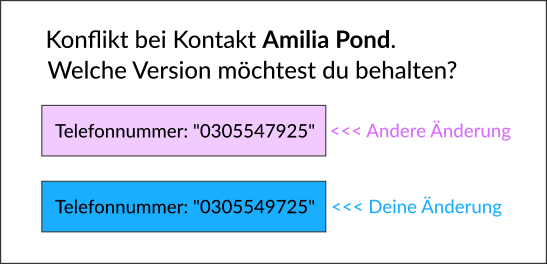
\includegraphics[width=0.8\textwidth]{Konfliktdialog}
    \grayRule
    \caption{Dialogfenster im Konfliktfall}
    \label{fig:dialog}
\end{figure}
Wurde beispielsweise Amilias Telefonnummer gleichzeitig bearbeitet, bildet der Dialog zwei Bereiche mit der Nummer in den unterschiedlichen Versionen ab.
Durch Klick auf die korrekte Nummer kann entschieden werden welche Version die richtige ist und behalten wird.